% Kapitel 3

\chapter{Data Efficiency in Neural Network-Based Image Segmentation}
\label{chap:data-efficiency}

Above all, the accuracy of neural networks is governed by three factors: problem complexity, number of network parameters, and size of the dataset. All of these factors contribute to accuracy in different ways and there is a complex interplay between them. To understand data efficiency, it is key to clearly understand these concepts. We will begin this chapter by exploring neural networks as function approximators. We still start with a simple example of a neural network and build an understanding of the four factors in general terms. After that, we will expand our example to include image segmentation.

Let us consider a statistical learning problem of estimating the 10-year risk of heart disease given age. In this case, there exists some unknown underlying dependency between age and risk of heart disease. However, there is no way to know what this function is. All we can do is collect a set of data points and try to approximate a function that explains those data points. In other words, we want to find a curve that tries to minimize some criterion that takes into account the distance between the curve and the collected data points.

TODO also mention noise

However, we have to make some choices before we try to fit a function. Namely, we have to choose how complex our curve should be. The simplest curve we could use is a line --- a simple linear regression. A line is defined by two parameters, its slope $\theta_1$ and intersect $\theta_2$:

\begin{equation}
	f(x) = \theta_1 x + \theta_0
\end{equation}

Here, $f(x)$ is our regression model. Our goal is to find the optimal values of $\alpha$ and $\beta$ that best explain the collected data samples in the form of $(x_i, y_i)$. We can do so by minimizing the mean squared distance between the line and each data point:

\begin{equation}
	\min_{\theta_1, \theta_0} \sum_{i=1}^N (y_i - f(x_i))
\end{equation}

Given a set data points, we will use the above equations to fit a line between them. In \figref{fig:slr-points} we show this line for a different number of datapoints. As can be seen, the number of samples impacts the results drastically. As is intuitive, more samples gives us a line that better matches the real data distribution.

\begin{figure}[h!]
 \hfill
 \subfloat{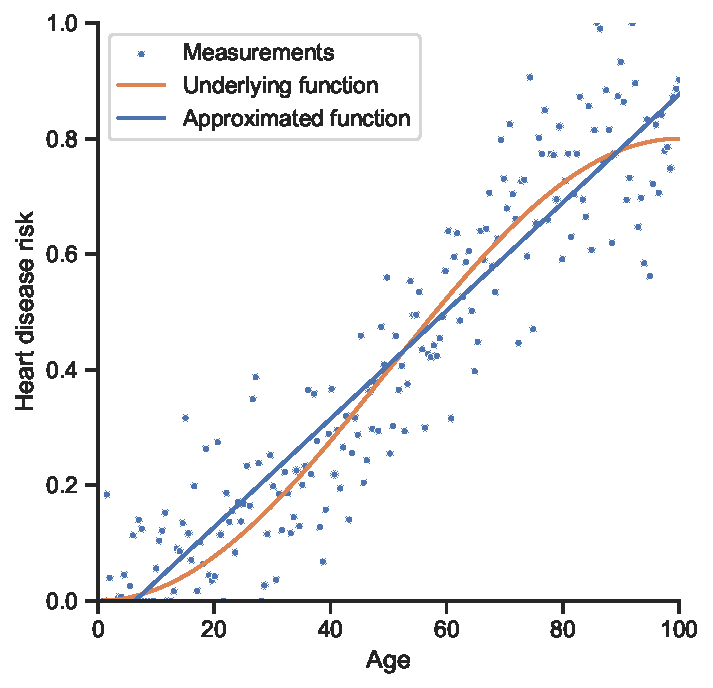
\includegraphics[width=0.5\linewidth]{images/3/heart_disease_risk}}
 \hfill
 \subfloat{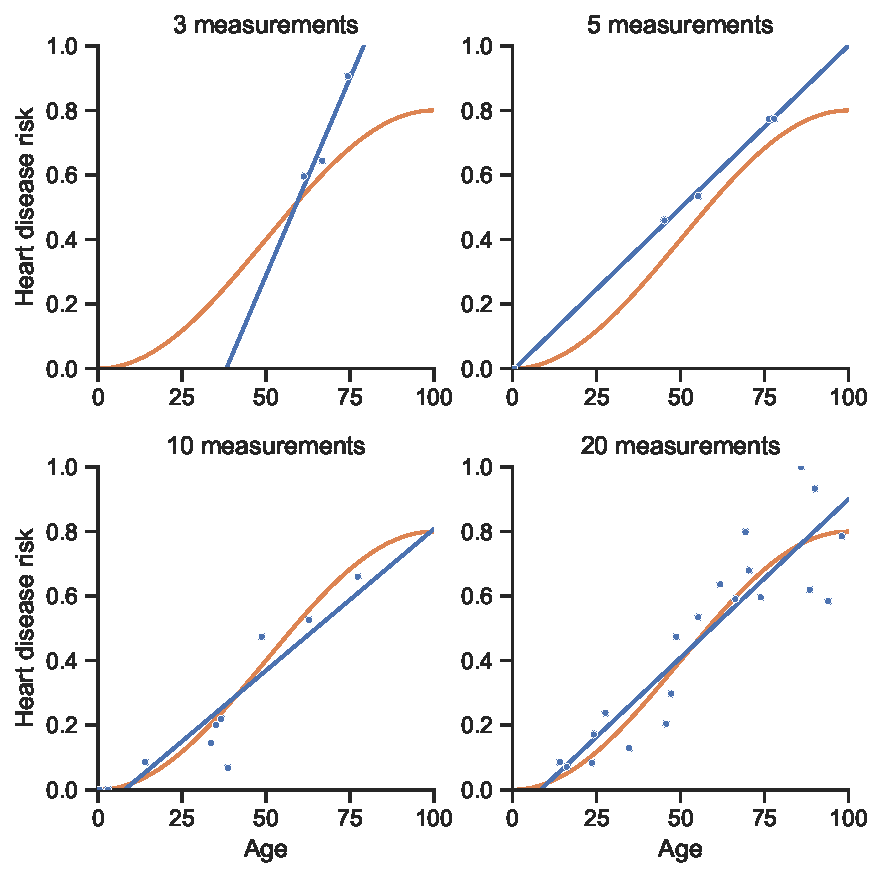
\includegraphics[width=0.5\linewidth]{images/3/heart_disease_risk_samples}}
 \hfill
 \label{fig:t1-t2-example}
 \caption{A simulated example of heart disease risk prediction using simple linear regression. The plots on the right show how the approximated function depends on the sample size.}
\end{figure}

Clearly, having only three points results in an approximated function that does not match the underlying one. As we increase the sample size, the approximated function becomes much closer to the underlying one. However, note that even for 20 measurements, the linear function differs from the underlying one. The underlying function is a non-linear cosine function. Even with infinitely many data points, our function will never approximate the underlying function perfectly with just two parameters.

To overcome this, we need a more complex model. We can think of our regression so far as fitting a polynomial function to our dataset. For the initial example, we have used polynomials with a degree of 1 --- lines. We can generalize our function to an $n$-degree polynomial as:

\begin{equation}
	f(x) = \theta_n x^n + \theta_{n-1}x^{n-1} + \cdots + \theta_1 x + \theta_0
\end{equation}

To model heart disease risk, we will choose a polynomial degree $n$ and minimize the mean squared distance to obtain $\theta_n$ through $\theta_0$. By increasing the degree increasing the complexity of the model, i.e. the model will be able to represent more complex curves than simple lines. We can observe what happens when we choose degrees 2, 3, or 5 in \figref{fig:reg-deg-2}.

\begin{figure}[h!]
 \centering
 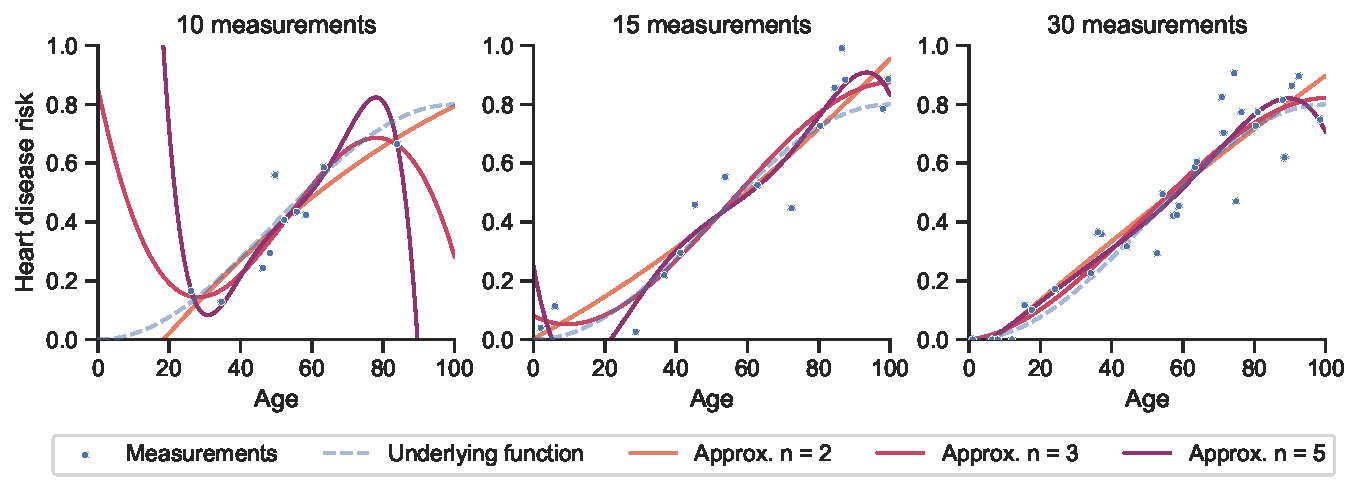
\includegraphics[width=\linewidth]{images/3/heart_disease_risk_samples_degrees}
 \caption{Fitting a polygonal function of various degrees on three different sample sizes.}
 \label{fig:reg-deg-2}
\end{figure}

When looking at the example with 10 measurements, we can see that for $n = 2$ the approximated polynomial follows the underlying function somewhat well. However, as we increase the degree the function quickly deteriorates. The function has enough freedom to closely fit between the 10 points, however, the 10 points are not enough to be representative of the underlying function. As we sample more points, we can see that even higher-degree polynomials can now approximate our function well. 

Thus, we may conclude that a model with more parameters is able to approximate more complex functions. However, to do so it requires more samples than a model with fewer parameters. This is an extension of the \textbf{bias---variance tradeoff}. 

discuss regularization, sample complexity

TODO Tie in with overfitting, bias variance tradeoff






When segmenting liver tumors in CT image, an expert, given a voxel location and image, can map each location to a probability of encountering a liver tumor on that image. They do so based on experience, intuition, and complex models of the real world including anatomy, pathology, biological processes of cancerous cell multiplication, understanding of how different vascular systems propagate contrast to cancerous and normal cells, etc. It is computationally infeasible to model these processes directly, so instead we opt for sampling a set of CT images and approximating the underlying processes as a continuous function.

The sampled points are in the form of $(I(A), M(A))$ i.e. an image and segmentation map pair, as labeled by an expert. If we consider the image and segmentation map to be high-dimensional vectors, we can think of both as existing in a high-dimensional space.


%At their core, neural networks are function approximators. Every voxel in a CT scan contains either normal tissue or a liver tumor. Cancerous cells multiply and grow according to biological processes and are thus localized in specific areas. Because the cancerous cells are supplied with blood by the hepatic artery, an injected contrast reaches them sooner than normal cells, causing them to appear brighter in the image. These are just a few of infinitely many processes that govern the true probability of a voxel containing cancerous tissue. All of these processes together form an exceedingly complex function that maps a voxel its true probability of containing cancerous tissue. The goal of a segmentation network is to approximate this natural function using a statistical model. 
%
%We may imagine a CT scan as a point that lies in a high-dimensional space, where each voxel value is one dimension of the point.
%
%
%In image segmentation, this 
%
%At their core, neural networks aim to replicate natural phenomena. Somewhere in the real world, there exists a natural process producing measurable changes. Cancerous liver cells receive their blood supply from the hepatic artery, while normal liver cells are supplied mostly by the portal vein. During a CT with contrast, the injected contrast enters the hepatic arterial system first and travels to the liver cells making them briefly appear brighter than surrounding normal cells. This is a physical process that produces a single measurement --- a CT image. We can collect many such images to form a liver tumor segmentation dataset. Given this dataset, we can task a neural network to approximate 
%
%
%At their core, neural networks approximate a function given a set of data points. The goal of the research community is that this approximate function is as close as possible to a real natural phen
%
%The ultimate goal of any machine learning researcher is to improve the accuracy of a model under some set of conditions. The conditions that impact the accuracy of neural networks be broadly classified into three groups: model design, training procedure, and data. These conditions have a dynamic interplay. The most reliable way to increase performance is by getting more and better quality data. Good is a necessary condition



% capacity -- complexity -- sample size dependency
% inductive bias
% other methods (check notes)

% https://www.frontiersin.org/articles/10.3389/fncom.2022.760085/full

